% Template for a Computer Science Tripos Part II project dissertation
\documentclass[12pt,a4paper,twoside,openright]{report}
\usepackage[pdfborder={0 0 0}]{hyperref}    % turns references into hyperlinks
\usepackage[margin=25mm]{geometry}  % adjusts page layout
\usepackage{graphicx}  % allows inclusion of PDF, PNG and JPG images
\usepackage{verbatim}
\usepackage{docmute}   % only needed to allow inclusion of proposal.tex
\usepackage{parskip}
\usepackage{todonotes}
\usepackage{listings}
\usepackage{amsmath}

\lstset{basicstyle=\ttfamily, breaklines=true}

\graphicspath{ {./images/} }

\newcommand{\quickwordcount}[1]{%
  \immediate\write18{texcount -1 -sum -merge -q #1.tex output.bbl > #1-words.sum }%
  \input{#1-words.sum}%
}

\raggedbottom                           % try to avoid widows and orphans
\sloppy
\clubpenalty1000%
\widowpenalty1000%

\renewcommand{\baselinestretch}{1.1}    % adjust line spacing to make
                                        % more readable

\begin{document}

\bibliographystyle{plain}


%%%%%%%%%%%%%%%%%%%%%%%%%%%%%%%%%%%%%%%%%%%%%%%%%%%%%%%%%%%%%%%%%%%%%%%%
% Title


\pagestyle{empty}

\rightline{\LARGE \textbf{Jiaxin Wang}}

\vspace*{60mm}
\begin{center}
\Huge
\textbf{A Recursive Recurrent Neural Network Decoder for Grammatical Error Correction} \\[5mm]
Computer Science Tripos -- Part II \\[5mm]
Emmanuel College \\[5mm]
\today  % today's date
\end{center}

%%%%%%%%%%%%%%%%%%%%%%%%%%%%%%%%%%%%%%%%%%%%%%%%%%%%%%%%%%%%%%%%%%%%%%%%%%%%%%
% Proforma, table of contents and list of figures

\pagestyle{plain}

\chapter*{Proforma}

{\large
\begin{tabular}{ll}
Candidate Number:   & -                       \\
Project Title:      & A Recursive Recurrent Neural Network \\
 & Decoder for Grammatical Error Correction \\
Examination:        & Computer Science Tripos -- Part II, 2022  \\
Word Count:         & \quickwordcount{diss}\footnotemark[1] \\
Code line count:    & 1127 \\
Project Originator: & - \\
Supervisor:         & Dr Zheng Yuan, Dr Christopher Bryant
\end{tabular}
}
\footnotetext[1]{This word count was computed
by \texttt{detex diss.tex | tr -cd '0-9A-Za-z $\tt\backslash$n' | wc -w}
}
\stepcounter{footnote}


\section*{Original Aims of the Project}

-


\section*{Work Completed}

-

\section*{Special Difficulties}

-
 
\newpage
\section*{Declaration}

I, Jiaxin Wang of Emmanuel College, being a candidate for Part II of the Computer
Science Tripos, hereby declare that this dissertation and the work described in 
it are my own work, unaided except as may be specified below, and that the dissertation
does not contain material that has already been used to any substantial
extent for a comparable purpose.

\bigskip
\leftline{Signed [signature]}

\medskip
\leftline{Date [date]}

\tableofcontents

\listoffigures

\newpage
\section*{Acknowledgements}

-

%%%%%%%%%%%%%%%%%%%%%%%%%%%%%%%%%%%%%%%%%%%%%%%%%%%%%%%%%%%%%%%%%%%%%%%
% now for the chapters
\listoftodos

\pagestyle{headings}

\chapter{Introduction}

This project concerns my implementation of a \textit{recursive recurrent neural network} model (R\textsuperscript{2}NN) proposed by Liu et al. (2014) \cite{r2nn} This is to be integrated in a statistical machine translation (SMT) system to attempt the task of grammatical error correction. \todo[inline]{More details}

\section{Motivation}

Grammatical Error Correction (GEC) is the task of producing a grammatically correct sentence given a potentially erroneous text while preserving its meaning. The main motivation behind this task lies in its role in helping learners of a foreign language understand the language better. In addition, native speakers can make use of such GEC tools to avoid mistakes in their writing. Being an ESL (English as a second language) learner myself, I would like to investigate models that can be used for the task of GEC in English, and I hope that it can benefit people who may find GEC tools useful.


\section{Problem Overview}

The task of Grammatical Error Correction can be seen as a machine translation process, where the input is a text which may contain grammatical errors, and the output is an error-free text. This project uses a statistical machine translation (SMT) approach to solve GEC.

A recursive recurrent neural network (R\textsuperscript{2}NN) was proposed by Liu et al. (2014) \cite{r2nn} for SMT. The goal of this project is to implement the proposed model to be used for GEC. The model should aim to correct all types of errors, namely grammatical, lexical, and orthographical errors. Its performance will be evaluated against a baseline SMT system, Moses\cite{moses}.


\section{Related Work}
-

\chapter{Preparation}

\section{Starting Point}

This project is based on the idea presented in the paper \textit{A Recursive Recurrent Neural Network for Statistical Machine Translation} \cite{r2nn}. An R\textsuperscript{2}NN model was proposed, but the implementation details are not given in the paper.

The Part IB Computer Science Tripos course Artificial Intelligence\footnote{https://www.cl.cam.ac.uk/teaching/2021/ArtInt/} gives an introduction to neural networks and explains how forwarding and backpropagation works. Prior to this project I did not have any coding experience with neural networks. I have found it useful to follow the coding examples on PyTorch\footnote{https://pytorch.org/tutorials/} website.

An example SMT system is available on Moses\footnote{https://www.statmt.org/moses/?n=Moses.Baseline} website. It provides a detailed tutorial on how to install Moses, how to prepare corpus and how to train the SMT.


\section{Theory}

\subsection{SMT system}
A typical SMT system consists of four main components: The language model (LM), the translation model (TM), the reordering model and the decoder\cite{yuan2017phd}. The LM computes the probability of a given sequence being valid. The TM builds a translation table which contains mappings of words/phrases between source and target corpora. The reordering model learns about phrase reordering of translation. The decoder finds a translation candidate who is most likely to be the translation of the source sentence. In the task of GEC, this would be the most probable correction to the original erroneous sentence.

\todo[inline]{Level of detail?}


\subsection{Moses SMT}
The Moses baseline system uses KenLM as the language model. For the translation model, it uses GIZA++ to obtain a word alignment model. The model should be trained to produce a phrase table and associated scores. Reordering tables are also created during this process. Eventually, the Moses decoder will find the best translation candidate given input based on the scores it calculated in previous stages.

\subsection{Feedforward Neural Network}
A feedforward neural network consists of three parts: an input layer, one or more hidden layers, and an output layer. In a feedforward neural network, data only flows in one direction (forward) from input to output. Figure \ref{fig:fnn} shows an example of a feedforward neural network with one hidden layer.

\begin{figure}[ht]
\centering
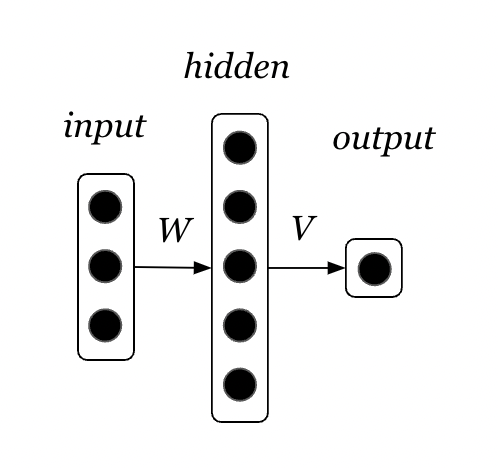
\includegraphics[width=0.3\textwidth]{images/fnn.png}
\caption{Example of a feedforward neural network}
\label{fig:fnn}
\end{figure}

\subsection{Recurrent Neural Network (RNN)}
Recurrent neural networks are usually used to deal with sequences. They allow access to the input data as well as past data to compute the next state. As shown in Figure \ref{fig:rnn}, the hidden layer $h_t$ is computed using both input $x_t$ at time $t$ and the hidden state $h_{t-1}$ which contains the history information from time 0 to $t-1$. For each timestep $t$, the hidden state can be expressed as:
\[ h_t = Wx_t + Uh_{t-1} \]

\begin{figure}[ht]
\centering
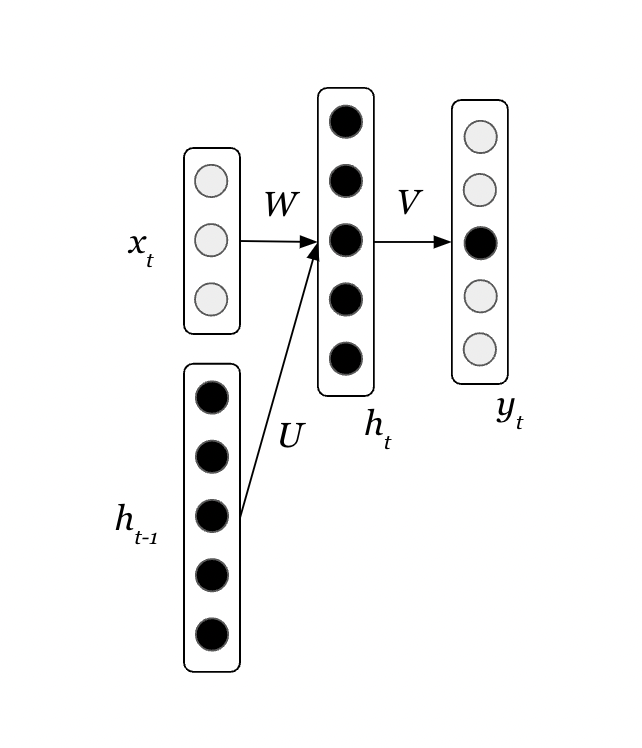
\includegraphics[width=0.4\textwidth]{images/rnn.png}
\caption{Example of a recurrent neural network (RNN)}
\label{fig:rnn}
\end{figure}


\subsection{Recursive Neural Network (RvNN)}
A recursive neural network has a tree-like structure. Figure \ref{fig:rvnn} illustrates an example of a basic RvNN architecture. The parent node representation is computed from its child nodes' representation as follows:
\[ p_{n, n+1} = f(W[x_n; x_{n+1}]) \]
where $f$ is the activation function. The same weight matrix $W$ will be applied recursively over the input.

\begin{figure}[ht]
\centering
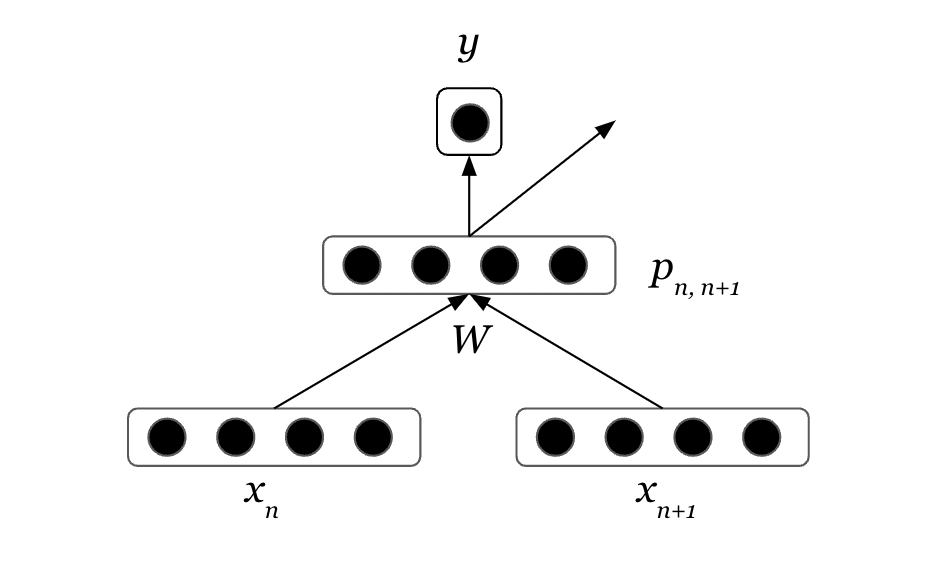
\includegraphics[width=0.6\textwidth]{images/rvnn.png}
\caption{Example of a recursive neural network (RvNN)}
\label{fig:rvnn}
\end{figure}


\subsection{\texorpdfstring{Recursive Recurrent Neural Network (R\textsuperscript{2}NN)}{Recursive Recurrent Neural Network (R2NN)}}
The R\textsuperscript{2}NN proposed by Liu et al.\cite{r2nn} combines the features of RvNN and RNN. It has a tree-like structure similar to RvNN, with recurrent vectors added to integrate global information. As shown in Figure \ref{fig:r2nn}, $s^{[l, m]}$ and $s^{[m, n]}$ is the representation of child nodes $[l, m]$ and $[m, n]$. The recurrent input vectors, $x^{[l, m]}$ and $x^{[m, n]}$ are added to the two child nodes respectively. They encode the global information, such as language model scores and distortion model scores. A third recurrent input vector $x^{[l, n]}$ is added to the parent node $[l, n]$. The parent node representation is computed as
\[ s_j^{[l, n]} = f(\sum_{i} \hat{x}_i^{[l, n]}w_{ji}) \]
where $\hat{x}$ is the concatenation of vectors $[x^{[l, m]}; s^{[l, m]}; x^{[m, n]}; s^{[m, n]}]$, and $f$ is the $HTanh$ function. The output, $y^{[l, n]}$, is computed as
\[ y^{[l, n]} = \sum_{j} ([s^{[l, n]}; x^{[l, n]}])_{j}v_j \]


\begin{figure}[ht]
\centering
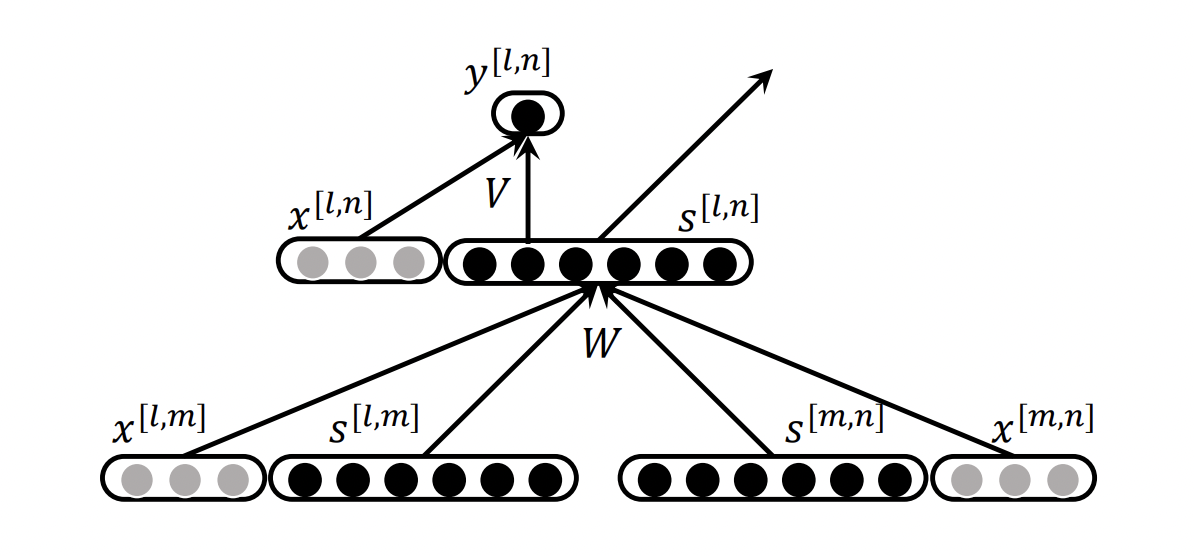
\includegraphics[width=0.6\textwidth]{images/r2nn.png}
\caption{Recursive recurrent neural network (Liu et al., 2014, p.1494)}
\label{fig:r2nn}
\end{figure}


\section{Requirement Analysis}

Based on the Project Structure section from my project proposal, the following requirements have been identified:

\textbf{Data preprocessing}
\begin{itemize}
    \item Data should be prepared in a form that is accepted by Moses SMT and R\textsuperscript{2}NN SMT
    \item Preprocessing should be done carefully to avoid accidentally correcting some of the grammatical errors 
    
    \begin{itemize}
        \item E.g. capitalisation errors may go undetected if all sentences are lowercased during data preprocessing
    \end{itemize}
\end{itemize}

\textbf{Moses SMT for GEC}
\begin{itemize}
    \item A language model should be trained to model the probability of a given sentence being valid
    \item A translation model should be trained to construct a phrase translation table
    \item A reordering model should be trained to learn the reordering of phrases
    \item With the above three models and Moses decoder, a complete Moses SMT system should be built
\end{itemize}

\textbf{R\textsuperscript{2}NN SMT for GEC}

Following the R\textsuperscript{2}NN paper by Liu et al.\cite{r2nn},
\begin{itemize}
    \item Phrase pair embeddings (PPE) should be learned by building a one-hidden-layer neural network and a recurrent neural network
    \item A recursive recurrent neural network (R\textsuperscript{2}NN) should be built and used as a decoder
\end{itemize}

\textbf{Evaluation}
\begin{itemize}
    \item The performance of both SMT systems should be evaluated using F0.5 scores
\end{itemize}

\section{Choice of Tools}

\subsection{Programming Language}

Python is chosen to be the main programming language as it provides many libraries that are commonly used for natural language processing. For this project I will be using \texttt{python 3.8} and PyCharm as my IDE.

\subsection{Libraries}
\textbf{PyTorch} \\
The \texttt{PyTorch}\footnote{https://pytorch.org/} library is one of the most popular machine learning frameworks. There are other similar libraries (such as \texttt{TensorFlow}) but I find \texttt{PyTorch} tutorials are easier to follow.

\textbf{NumPy} \\
My project is likely to involve statistical processing. I would be using the \texttt{NumPy}\footnote{https://numpy.org/} library for this purpose.

\textbf{pandas} \\
\texttt{pandas}\footnote{https://pandas.pydata.org/} is a powerful library for processing tabular data. This would be used to manipulate phrase tables in my project.

\subsection{Dataset}
The dataset introduced in BEA 2019 Shared Task\cite{bryant-etal-2019-bea} will be used in this project. I chose the corpora (\textbf{FCE v2.1}) which is immediately downloadable from the website\footnote{https://www.cl.cam.ac.uk/research/nl/bea2019st/\#data} to start with. The corpora have been standardised to be easily evaluated by ERRANT\cite{bryant-etal-2017-automatic,felice-etal-2016-automatic}. ERRANT is a toolkit used to annotate parallel data and compare hypothesis against reference to produce various evaluation metrics including F0.5 score. I may request other corpora as an extension of my project.

For language model training, I will be using the \textbf{One Billion Word} dataset\cite{one-billion-word}. This is a dataset used for language modeling and is available on GitHub\footnote{https://github.com/ciprian-chelba/1-billion-word-language-modeling-benchmark}.

\subsection{Version Control and Backup}
Git will be used for version control. The entire project, including all the written code and my dissertation, will be pushed to GitHub regularly.

\chapter{Implementation}
This chapter describes the implementation of a Moses baseline SMT system and a R\textsuperscript{2}NN SMT system. Since the main purpose of this project is to compare the performance of our R\textsuperscript{2}NN decoder against Moses decoder, the R\textsuperscript{2}NN system should use the same language model, translation model and reordering model as Moses. For the translation model, the R\textsuperscript{2}NN paper\cite{r2nn} proposed a \textit{translation confidence based phrase pair embedding} (TCBPPE) to be used with the R\textsuperscript{2}NN decoder. The TCBPPE will be based on a phrase table which is produced by Moses translation model. In the end, the R\textsuperscript{2}NN decoder will make use of language model scores, translation model scores, reordering model scores from Moses as well as TCBPPE to find the best translation candidate.

\begin{figure}[ht]
\centering
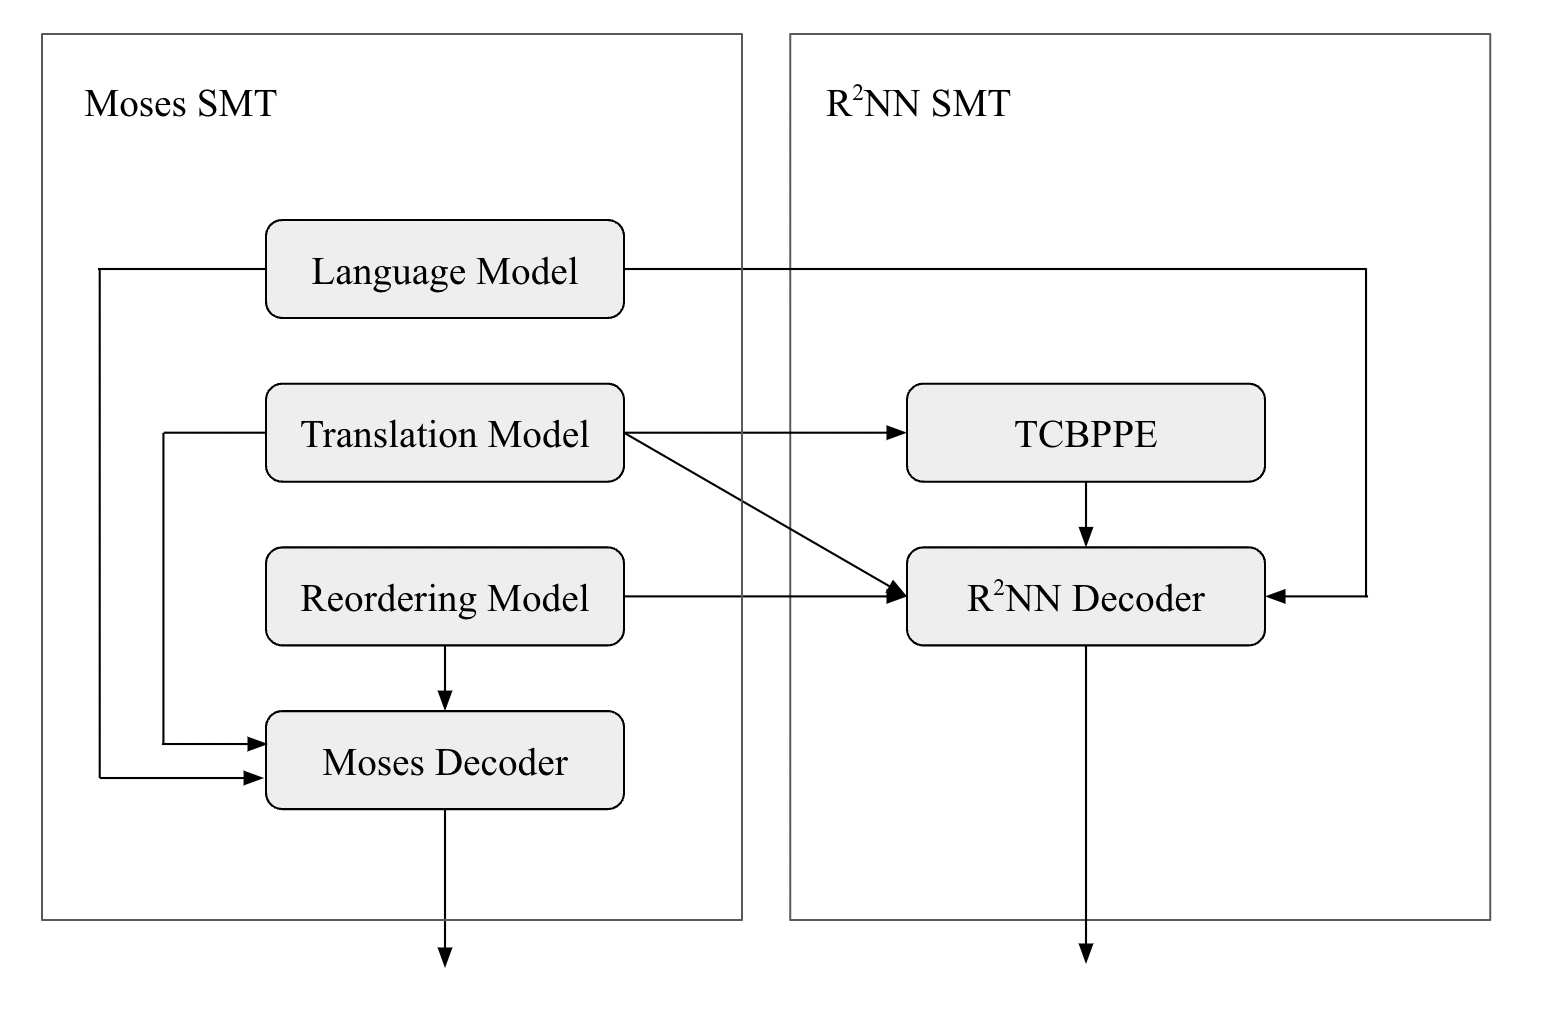
\includegraphics[width=0.8\textwidth]{images/overview_moses_r2nn.png}
\caption{Overview of Moses SMT and R\textsuperscript{2}NN SMT}
\label{fig:moses_r2nn}
\end{figure}

\section{Repository Overview}
-

\section{Setup}

\subsubsection{FCE Dataset}

The FCE dataset was provided in m2 format. However, Moses requires parallel data which is aligned at the sentence level. An example taken from the m2 file looks like this:

\texttt{S Her friend Pat had explained the whole story at her husband .\\
A 8 9|||R:PREP|||to|||REQUIRED|||-NONE-|||0}

[This means that for source sentence S, the word at position 8 to 9 (\texttt{at}) should be corrected to \texttt{to}.]

The m2 format needs to be converted to sentence-aligned data to be used by Moses. Two files are generated from this, where the source file contains\\
\texttt{Her friend Pat had explained the whole story at her husband .}

and the target file contains\\
\texttt{Her friend Pat had explained the whole story to her husband .}

\subsubsection{One Billion Word Dataset}

I downloaded the One Billion Word dataset for language model training. However, the files were too large to be handled by my machine. Since the dataset consists of fifty files, I decided to randomly choose 10 files from them and concatenated these files to be used in language model training. 


\section{Moses Baseline}

\begin{figure}[ht]
\centering
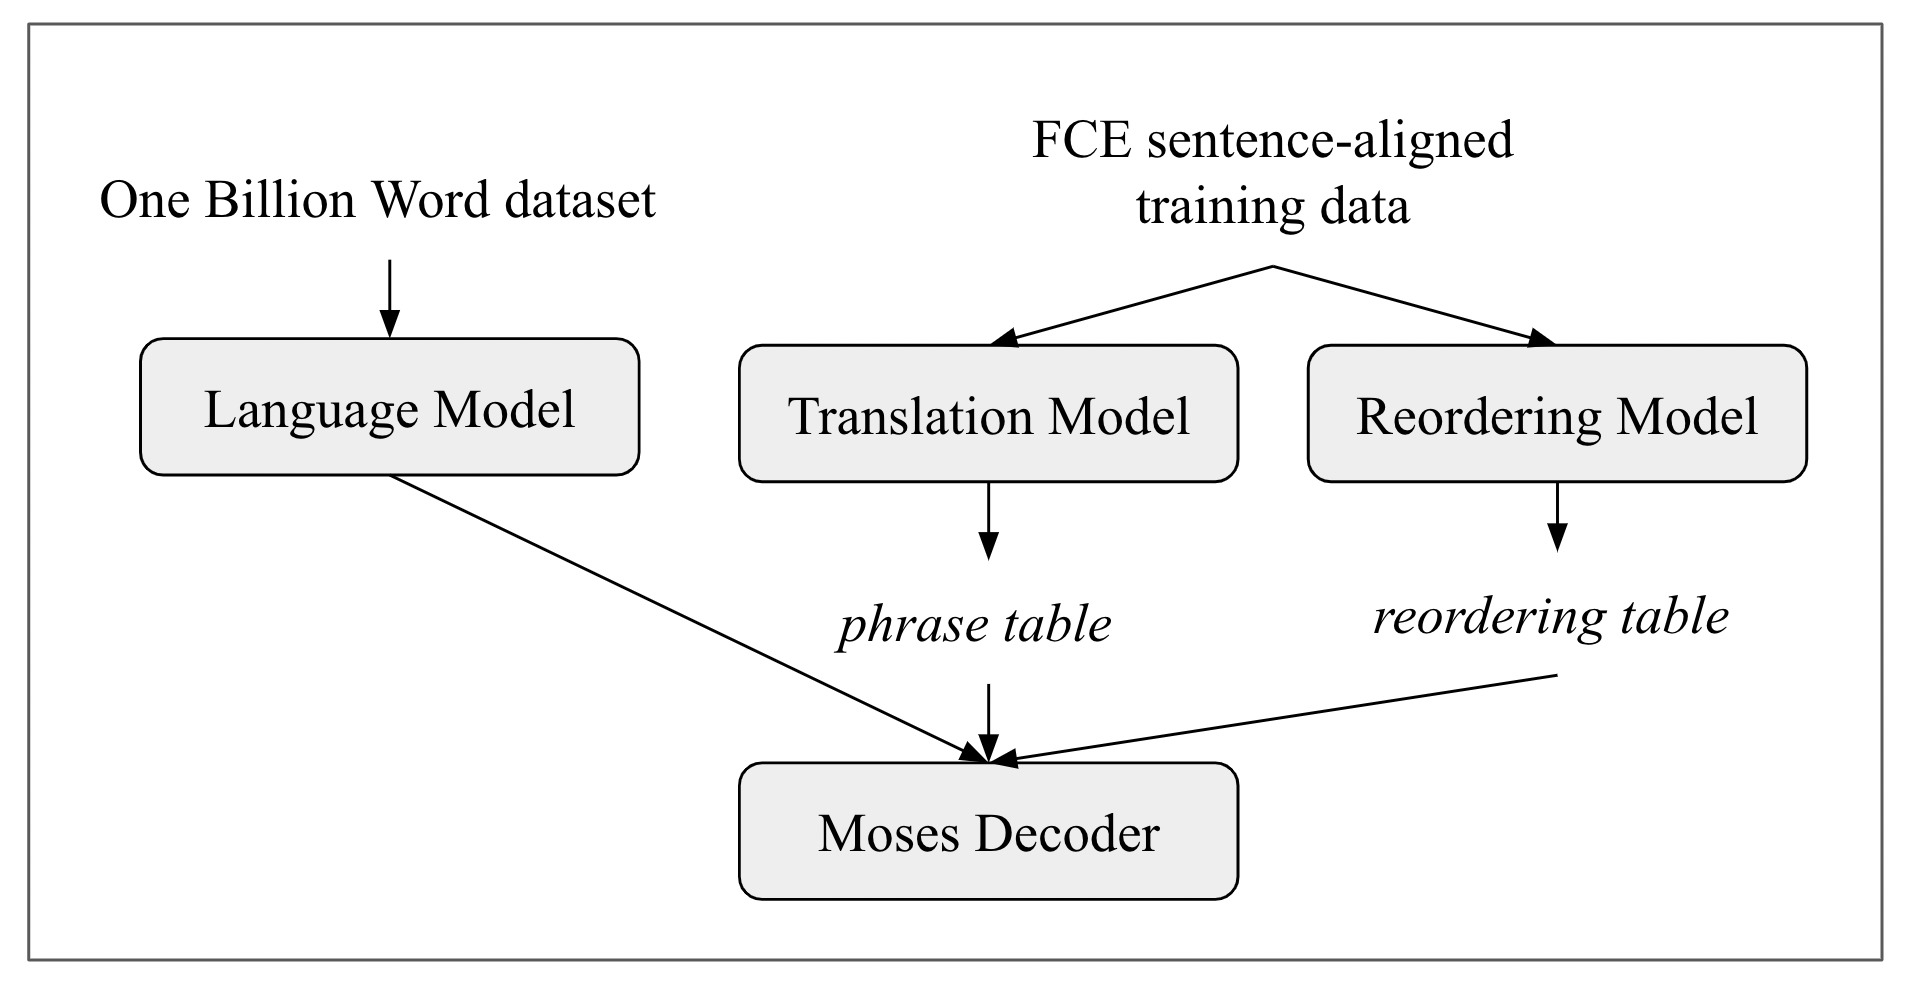
\includegraphics[width=0.8\textwidth]{images/moses_pipeline.png}
\caption{Overview of Moses SMT}
\label{fig:moses_pipeline}
\end{figure}

\subsection{Language Model}
The One Billion Word dataset is used for language model training. In the R\textsuperscript{2}NN paper, a 5-gram language model is used. Here, I used KenLM which came with Moses installation to train a 5-gram language model. An example query of the trained language model looks like this:
\todo[inline]{Example query of LM}

\subsection{Translation Model and Reordering Model}
The translation model is trained with FCE sentence-aligned data. There are three components in translation model training: word alignment, phrase extraction and scoring. Word alignment is obtained using GIZA++, a toolkit to train word alignment models. Phrases are then extracted from our training files and a phrase table is produced. The phrase table contains phrase translation pairs and the scores associated with each pair.

\begin{table}[h!]
\centering
\begin{tabular}{ |c|c|c|c|c| } 
 \hline
 source & target & scores & alignment & counts \\ [0.5ex] 
 \hline
 As we & As we & 1 0.901657 0.846154 0.90511 & 0-0 1-1 & 11 13 11\\
 As we & We & 0.00115075 1.68879e-05 0.0769231 0.0153198 & 1-0 & 869 13 1\\
 As we & as we & 0.0212766 0.00117032 0.0769231 0.00482726 & 0-0 1-1 & 47 13 1\\
 \hline
\end{tabular}
\caption{Phrase table from Moses}
\label{table:phrase_table}
\end{table}

A distance-based reordering model is then built, and a reordering table is created. Finally, Moses decoder would make use of the language model, the phrase table as well as the reordering table. Given a source sentence, the Moses decoder will output the best translation candidate based on the scores from the above models. 

\section{\texorpdfstring{R\textsuperscript{2}NN}{R2NN} SMT}

\begin{figure}[ht]
\centering
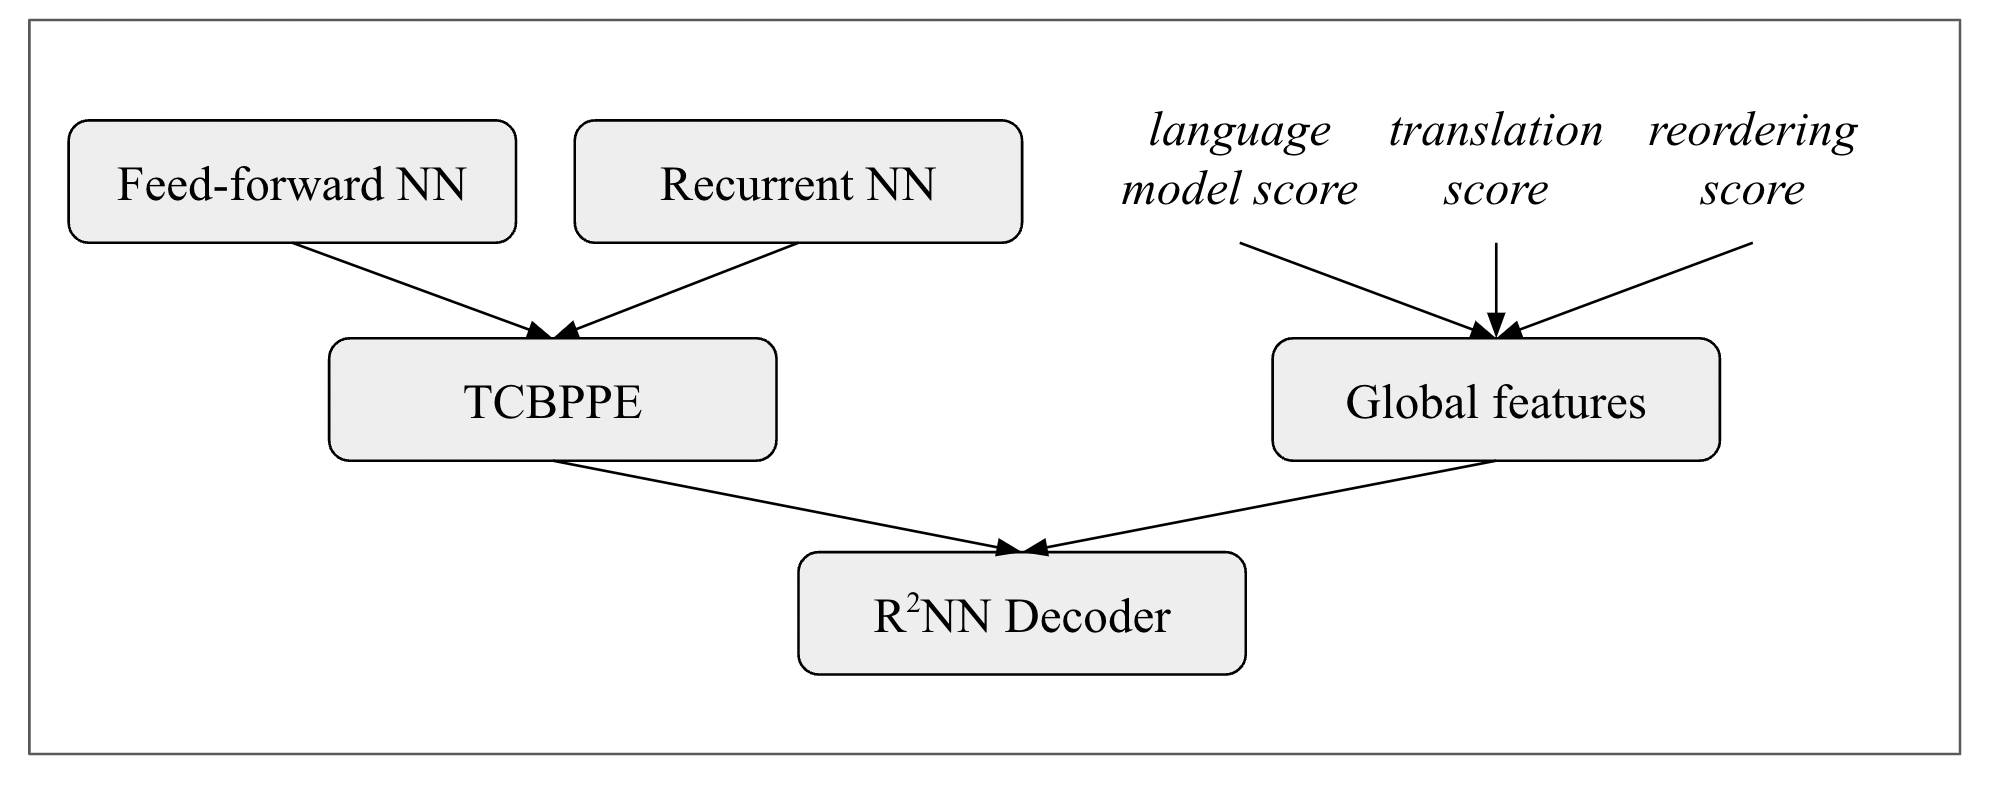
\includegraphics[width=1\textwidth]{images/r2nn_pipeline.png}
\caption{Overview of R\textsuperscript{2}NN SMT}
\label{fig:r2nn_pipeline}
\end{figure}

The R\textsuperscript{2}NN SMT consists of three parts: translation confidence based phrase pair embedding (TCBPPE), global features, and a R\textsuperscript{2}NN decoder.

\subsubsection{TCBPPE}
A phrase pair embedding is a vector representation which encodes the meaning of a phrase pair. Recall that our R\textsuperscript{2}NN model has a tree structure, where each node has a representation vector $s$ and a recurrent vector $x$. The TCBPPE is to be used as the representation vector $s$ and it is used to generate the leaf nodes of the derivation tree. 

The phrase pair embedding is split into two parts: translation confidence with sparse features and translation confidence with recurrent neural network. These two vectors will be obtained separately, and will be concatenated to be used as the representation vector $s$ in the R\textsuperscript{2}NN.

\subsubsection{Global features}
The global features encode global information that cannot be generated by child representations. It includes language model scores, translation scores and reordering scores which are obtained from Moses. These scores are concatenated together to be used as recurrent vectors $x$ to the R\textsuperscript{2}NN model.

\subsubsection{R\textsuperscript{2}NN decoder}
The recursive recurrent neural network (R\textsuperscript{2}NN) will be used as a decoder to find the best translation candidate. For an input sentence, the decoder would construct a tree based on phrases in the sentence. An output score will be computed based on TCBPPE, global features and the structure of the tree. The translation candidate that gives the highest score will be taken as the best translation candidate.

\subsection{TCBPPE: Sparse Features}

\begin{figure}[ht]
\centering
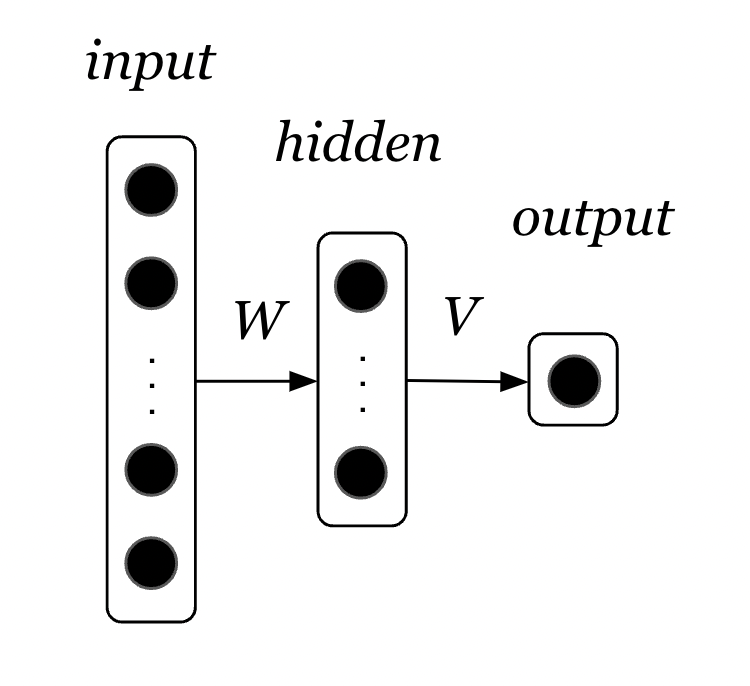
\includegraphics[width=0.3\textwidth]{images/one_hidden_layer.png}
\caption{Structure of one-hidden-layer feedforward neural network}
\label{fig:one_hidden_layer}
\end{figure}

A one-hidden-layer feedforward neural network is used to get a translation confidence score using sparse features. The structure of the network is shown in Figure \ref{fig:one_hidden_layer}. Following the R\textsuperscript{2}NN paper\cite{r2nn}, the size of the hidden layer is set to 20. The size of the input layer is 200,001. By training the network, we obtain hidden matrix $W$ of size 200,001 by 20. $W$ will be used as phrase pair embedding matrix for sparse features (\texttt{ppe\_sparse}). The goal is to find the $W$ that gives the best phrase pair embedding.

Firstly, the training data (sentences) need to be encoded as one-hot like data to be used as input to the network. The top 200,000 most frequent phrase pairs in the Moses translation table are selected, each to be a feature itself, and an additional feature is used for all the other phrase pairs. For each sentence pair (source-target) in the training data, it needs to be encoded as a vector of length 200,001 consisting of 0s and 1s, where the position $i$ in the vector contains a 1 if and only if the $i$\textsuperscript{th} most frequent phrase pair is found in this sentence pair. An example taken from the training file:

[Source sentence]
\texttt{What she would do ?}

[Target sentence]
\texttt{What would she do ?}

[Encoded vector]
\texttt{[$\underset{0}{0}, ..., \underset{39}{1}, ..., \underset{200000}{1}$]}

A 0 at position 0 means that the most frequent phrase pair does not exist in the sentence pair. A 1 at position 39 means that the 40\textsuperscript{th} most frequent phrase pair exists in the sentence pair. A 1 at position 200,000 means that the sentence pair contains a phrase pair that is not in the top 200,000 most frequent pairs.

\begin{table}[h!]
\centering
\begin{tabular}{ |c|c|c|c| } 
 \hline
 index & source & target & ... \\ [0.5ex] 
 \hline
 0 & . & . & ... \\ 
 ... & ... & ... & ... \\ 
 39 & do & do & ... \\ 
 \hline
\end{tabular}
\caption{Top 200,000 phrase pairs}
\label{table:pt_top_exmaple}
\end{table}

One problem with this is that the resulting vector from sentence pairs are usually sparse vectors. To save memory, instead of storing the whole vector, the position indices of 1s in the vector are stored in a file named \texttt{phrase\_pair\_id} (i.e. the phrase pair ids used in each sentence pair are stored). When loading the sentence pairs as training data, it is easy to obtain the one-hot encoding of each sentence pair from \texttt{phrase\_pair\_id}.

The next step is to obtain the expected output for each input sentence pair. Since the TCBPPE encodes translation model information, it is reasonable to use the translation scores from Moses translation model. For each sentence pair $S\textrm{-}T$ containing phrase pairs $p_1, p_2, ..., p_n$, the expected output score is computed by
\[ score_{S\textrm{-}T} = \frac{\sum_n c_{p_n}}{n} \]
where $c_{p_n}$ is the average translation score for phrase pair $p_n$.

\begin{figure}[ht]
\centering
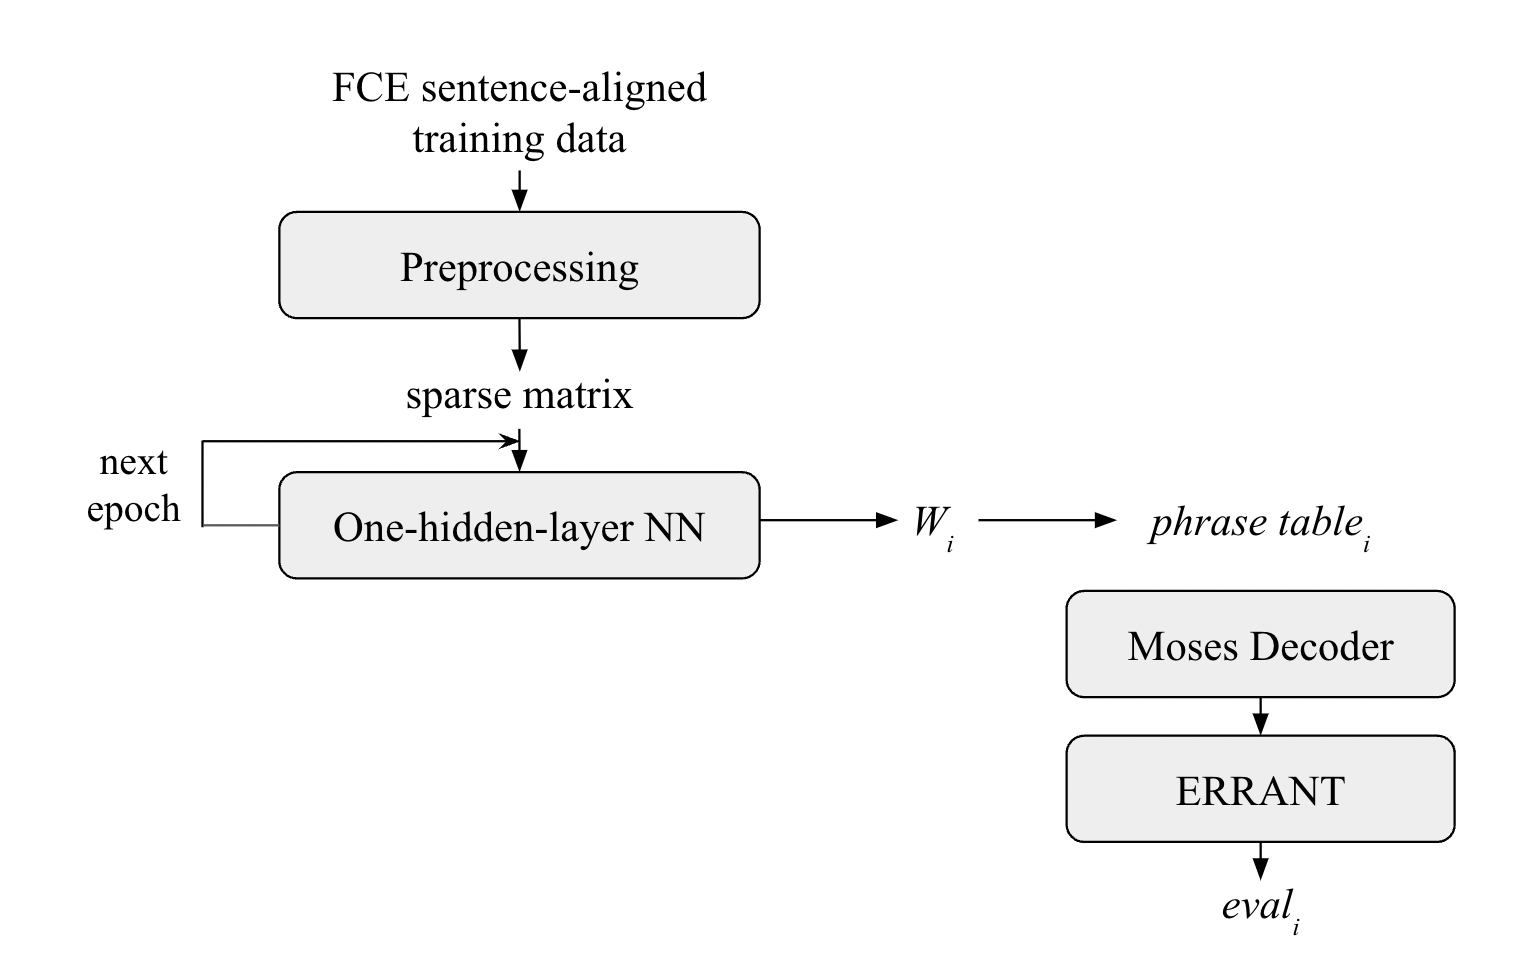
\includegraphics[width=0.8\textwidth]{images/sparse_pipeline.png}
\caption{Training pipeline of one-hidden-layer feedforward neural network}
\label{fig:sparse_pipeline}
\end{figure}


After obtaining the training dataset, we can train the neural network. The neural network will be trained for 10 epochs, where one epoch refers to one cycle of processing all the data in training set. After each epoch, the hidden matrix $W$ is stored. The $k^{th}$ row in $W$ will be used as the phrase pair embedding (sparse) for the top $k^{th}$ frequent phrase pair. That is, the embedding for the most frequent phrase pair is $W[0]$, and the embedding for phrase pairs that are not in the top 200,000 is represented by $W[200000]$.

We evaluate $W$ by updating the Moses phrase table: for each row (ppe) in $W$, we add the ppe as an additional feature to the phrase table. Then we pass the updated phrase table to Moses decoder and use ERRANT to evaluate the performance. Table \ref{table:sparse_5} and Table \ref{table:sparse_10} shows the evaluation result by ERRANT for training epoch 5 and training epoch 10 respectively. Among all the $W$ from epoch 1 to 10, 10-epoch $W$ gives the highest precision, recall and $F_{0.5}$ score. Hence, $W$ will be used as the ppe matrix for sparse features (\texttt{ppe\_sparse}).

\begin{table}[h!]
\centering
\begin{tabular}{ |c|c|c|c|c|c| } 
 \hline
 TP & FP & FN & Prec & Rec & F0.5 \\ [0.5ex] 
 \hline
 543 & 2366 & 4006 & 0.1867 & 0.1194 & 0.1677 \\ 
 \hline
\end{tabular}
\caption{ERRANT output (5 epochs)}
\label{table:sparse_5}
\end{table}

\begin{table}[h!]
\centering
\begin{tabular}{ |c|c|c|c|c|c| } 
 \hline
 TP & FP & FN & Prec & Rec & F0.5 \\ [0.5ex] 
 \hline
 545 & 2363 & 4004 & 0.1874 & 0.1198 & 0.1684 \\ 
 \hline
\end{tabular}
\caption{ERRANT output (10 epochs)}
\label{table:sparse_10}
\end{table}


\subsection{TCBPPE: Recurrent Neural Network (RNN)}

- Word embedding (fasttext vs word2vec)

\subsection{Global Features}

\subsection{Building \texorpdfstring{R\textsuperscript{2}NN}{R2NN}}
- Recursive neural network (RvNN)

- Recurrent input vectors

\section{Testing}

\chapter{Evaluation}

\chapter{Conclusion}


%%%%%%%%%%%%%%%%%%%%%%%%%%%%%%%%%%%%%%%%%%%%%%%%%%%%%%%%%%%%%%%%%%%%%
% the bibliography
\addcontentsline{toc}{chapter}{Bibliography}
\bibliography{refs}

%%%%%%%%%%%%%%%%%%%%%%%%%%%%%%%%%%%%%%%%%%%%%%%%%%%%%%%%%%%%%%%%%%%%%
% the appendices
\appendix

\chapter{Project Proposal}

% \chapter{Latex source}

% \section{diss.tex}
% {\scriptsize\lstinputlisting[language=TeX]{diss.tex}}

% \section{proposal.tex}
% {\scriptsize\verbatiminput{proposal.tex}}

% \chapter{Makefile}

% \section{refs.bib}
% {\scriptsize\verbatiminput{refs.bib}}


% \chapter{Project Proposal}

% \input{proposal}

\end{document}